\documentclass[t]{beamer}

% Load general definitions
% Preamble file - general definitions, package loading, etc.

%=================================
% Load packages
\usepackage{amssymb,amsmath}
\usepackage{graphicx}
\usepackage{url}
\usepackage{tikz}
\usetikzlibrary{mindmap,trees,arrows}
\usepackage{fancyvrb}
\usepackage[portuguese]{babel} 
\usepackage[utf8]{inputenc}
\usepackage{subfigure}
\usepackage{times}
\usepackage[T1]{fontenc}
\usepackage{cancel}
\usepackage{color}
\usepackage{listings}
\usepackage[document]{ragged2e}
\usepackage{physics}
\usepackage{amsmath}
\usepackage{tikz}
\usepackage{mathdots}
\usepackage{yhmath}
\usepackage{cancel}
\usepackage{color}
\usepackage{siunitx}
\usepackage{array}
\usepackage{multirow}
\usepackage{amssymb}
\usepackage{gensymb}
\usepackage{tabularx}
\usepackage{extarrows}
\usepackage{booktabs}
\usetikzlibrary{fadings}
\usetikzlibrary{patterns}
\usetikzlibrary{shadows.blur}
\usetikzlibrary{shapes}

%=================================
% Set mode
\mode<presentation>
{
	\usetheme{Madrid}
	\usecolortheme{structure}
	\useoutertheme{infolines}
	\setbeamercovered{invisible}
}

% Get rid of nav bar
\beamertemplatenavigationsymbolsempty

% Insert frame number at bottom of the page.
\usefoottemplate{\hfil\tiny{\color{black!90}\insertframenumber}} 

%=================================
% Define new commands

\newcommand\Real{{\mathbb{R}}}
%\newcommand{\vi}{\vspace{0.6\baselineskip}}
%\newcommand{\goodgap}{\hspace{\subfigtopskip}\hspace{\subfigbottomskip}}


% Equation environments
\newcommand{\beq}{\begin{equation}}
\newcommand{\eq}{\end{equation}}
\newcommand{\beqs}{\begin{equation*}}
\newcommand{\eqs}{\end{equation*}}
\newcommand{\beqn}{\begin{eqnarray}}
\newcommand{\eqn}{\end{eqnarray}}
% Bold variables
\newcommand{\mbf}[1]{\ensuremath{\mathbf{#1}}}
% Itemization
\newcommand{\bitem}{\begin{itemize}}
\newcommand{\eitem}{\end{itemize}}
\newcommand{\spitem}{\vskip 1em\item}
\newcommand{\bitems}{\begin{itemize}\item}
\newcommand{\benums}{\begin{enumerate}\item}
\newcommand{\eenum}{\end{enumerate}}
% color blocks
\newenvironment{colorblock}[2]{%
\setbeamercolor{block title}{#2}
\begin{block}{#1}}{\end{block}}
% Vertical spacing
\newcommand{\vone}{\vskip 1em}
\newcommand{\vhalf}{\vskip .5em}
% Frame environments
\newenvironment{ftst}[3][t]{%
\begin{frame}{environment=ftst,#1}
\frametitle{#2}
\framesubtitle{#3}}{\end{frame}}
\newenvironment{ftstf}[2]{
\begin{frame}[fragile,environment=ftstf]
\frametitle{#1}
\framesubtitle{#2}}{\end{frame}}
% colors
\definecolor{MyGray}{rgb}{0.5,0.5,0.5}
\definecolor{MyDBGray}{rgb}{0.1,0.1,0.4}
\definecolor{darkgreen}{rgb}{0,0.4,0}
\definecolor{black}{rgb}{0,0,0}
\def\defn#1{{\color{red} #1}}
% Footnote
\renewcommand{\thefootnote}{\alph{footnote}}
% Relaxed footnotes
\newcommand{\lfr}[1]{\let\thefootnote\relax\footnote{\tiny #1}}
% Verbatim environment - using FANCYVRB package
\DefineVerbatimEnvironment%
{rcode}{Verbatim}
{fontsize=\scriptsize}
% Verbatim environment - using LISTINGS package
%\lstnewenvironment{rcode} {\lstset{	language = R,
%									basicstyle = \scriptsize\ttfamily,
%									showspaces = false,
%									showstringspaces = false,
%									showtabs = false,
%									keywordstyle = \color{black}\bfseries,
%									commentstyle = \color{darkgreen},
%									numbers = none,
%									otherkeywords={	<-,
%													ggplot,
%													geom_boxplot,
%													facet_grid,
%													shapiro.test,
%													fligner.test,
%													glht,
%													with},
%									deletekeywords={data,
%													model,
%													residuals,
%													c,
%													axis,
%													default,
%													labels,
%													qq.text}}}%
%{}

% Specific definitions
\title[]{Banco de dados II}
\subtitle[]{Visão geral}
\author[]{Patrícia Lucas\\{\footnotesize }}
\institute{Bacharelado em Sistemas de Informação \\ IFNMG  - Campus Salinas}
\date{\scriptsize Salinas\\Agosto 2021}

\begin{document}

% cover page
\setbeamertemplate{footline}{}
\begin{frame}

\begin{center}
\includegraphics[width=.15\textwidth]{}
\end{center}
  \titlepage
  \begin{tikzpicture}[remember picture,overlay]
  \node[anchor=south east,xshift=-5pt,yshift=5pt] at (current page.south east) {\tiny Versão 1.2021};
  \node[anchor=south west,yshift=0pt] at (current page.south west) {
\includegraphics[width=.25\textwidth]{Logos/salinas_horizontal_jpg.jpg}};
  \end{tikzpicture}  
\end{frame}

% Main slides
\begin{ftst}{Mudanças do modelo industrial}{Ciência de dados}

\begin{figure}
    \centering
    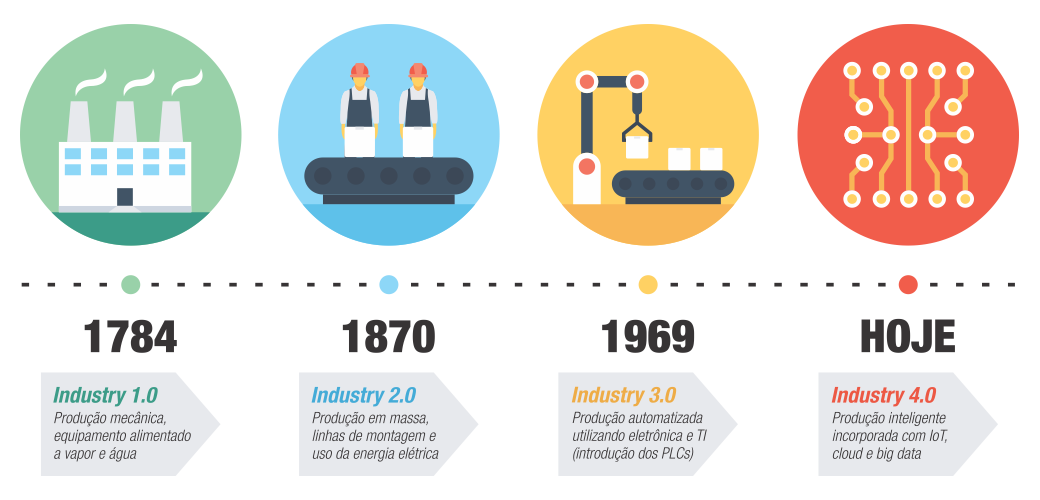
\includegraphics[scale=0.3]{Figuras/slide00_01.png}
\end{figure}
\vone
\vone
\vone
\vone
\vone
\vone
\scriptsize
Fonte da imagem: \href{https://bit.ly/2XHP0Pg}{\textcolor{blue}{https://bit.ly/2XHP0Pg}}
\end{ftst}

%===================================================================

\begin{ftst}{Indústria 4.0}{Ciência de dados}

\begin{figure}
    \centering
    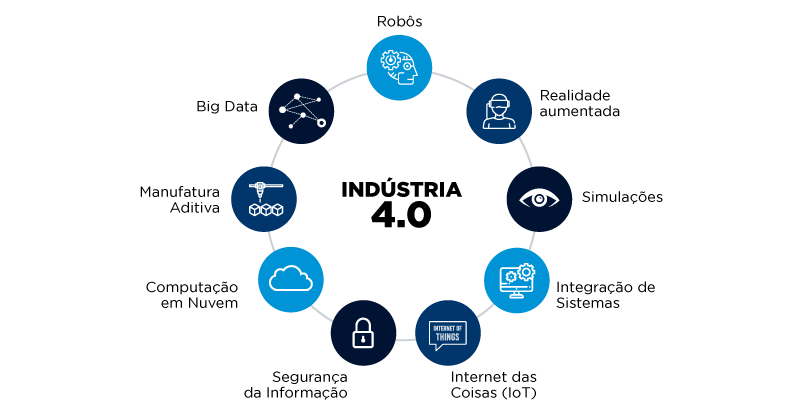
\includegraphics[scale=0.4]{Figuras/slide00_02.png}
\end{figure}
\vone
\vone
\scriptsize
Fonte da imagem: \href{https://bit.ly/2XHP0Pg}{\textcolor{blue}{https://bit.ly/3zeciu9}}
\end{ftst}

%===================================================================

\begin{ftst}{Indústria 4.0}{Ciência de dados}

\begin{itemize}
    \item A indústria 4.0 possui acesso fácil e a um custo baixo à dispositivos como robôs, câmeras, sensores e etc.
    \item Isso abre uma ampla gama de oportunidades para explorar em termos de coleta dados.
    \item O aumento da quantidade de dados é algo que está crescendo exponencialmente. \item A questão que fica é como esses dados são tratados e como realizar o conhecimento a partir dos dados de forma rápida e inteligente?
    \item Vindo de diferentes fontes e em diferentes formatos, existe uma enorme necessidade de processar esses dados, convertê-los em conhecimento e utilizá-los de forma proativa e preditiva, criando valor de conhecimento e construindo confiança digital.
\end{itemize}
\end{ftst}

%===================================================================

\begin{ftst}{Indústria 4.0}{Ciência de dados}

\begin{figure}
    \centering
    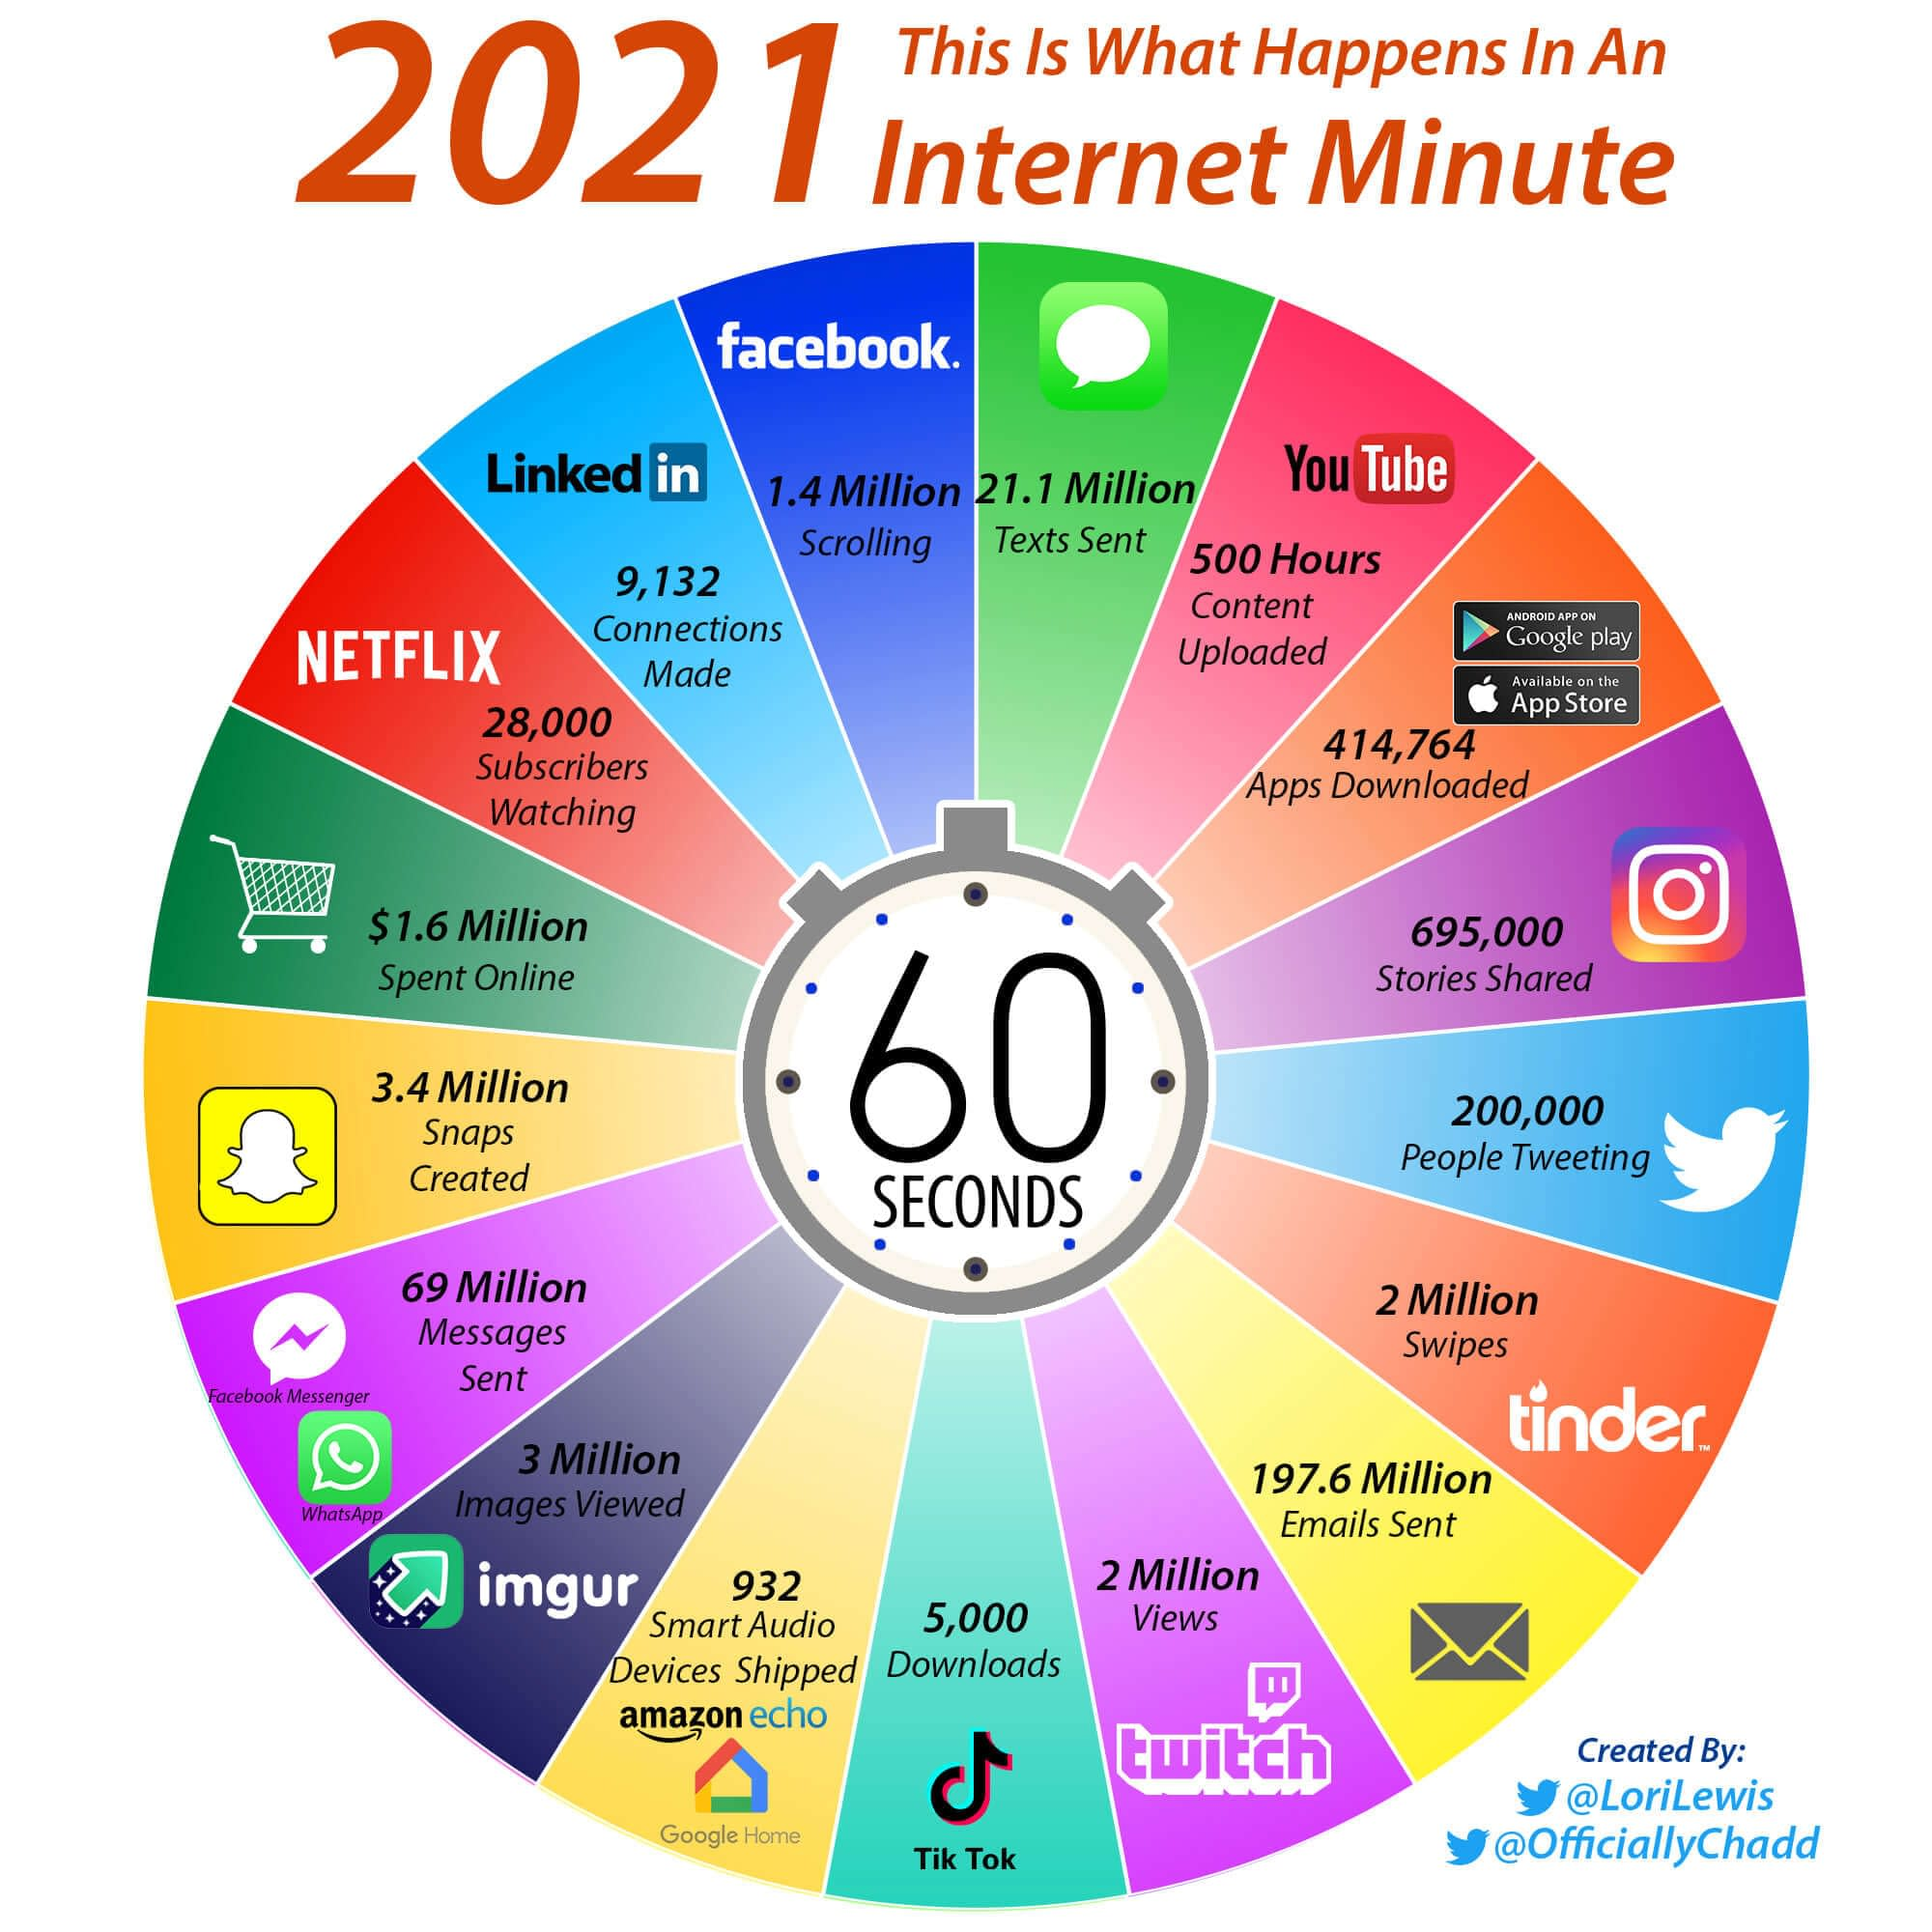
\includegraphics[scale=0.09]{Figuras/slide00_03.jpg}
\end{figure}

\scriptsize
Fonte da imagem: \href{https://bit.ly/3yeWkyD}{\textcolor{blue}{https://bit.ly/3yeWkyD}} 
 
Estatísticas da internet em tempo real: \href{https://www.internetlivestats.com/}{\textcolor{blue}{https://www.internetlivestats.com/}}

\end{ftst}


%===================================================================

\begin{ftst}{Dados e mais dados}{Ciência de dados}
\small
\begin{itemize}
    \item A economia está inevitavelmente se movendo em direção a produção de produtos e serviços baseados em tecnologias como inteligência artificial (IA), aprendizado de máquina e outros processos semelhantes controlados por computadores de alto desempenho.
    \item Todas essas tecnologias dependem da disponibilidade e do acesso aos dados.
    \item Os dados podem ser o novo bem mais valioso da economia moderna.
    \item Assim, terão um papel cada vez mais fundamental como parâmetro de competição, com muitas consequências para os negócios da atualidade.
    \item Os dados, além de serem indispensáveis para a IA, podem ser usados para criar modelos de negócios inovadores e e mercados inteiramente novos.
\end{itemize}

\end{ftst}

%===================================================================

\begin{ftst}{Importância econômica dos dados}{Ciência de dados}
\begin{figure}
    \centering
    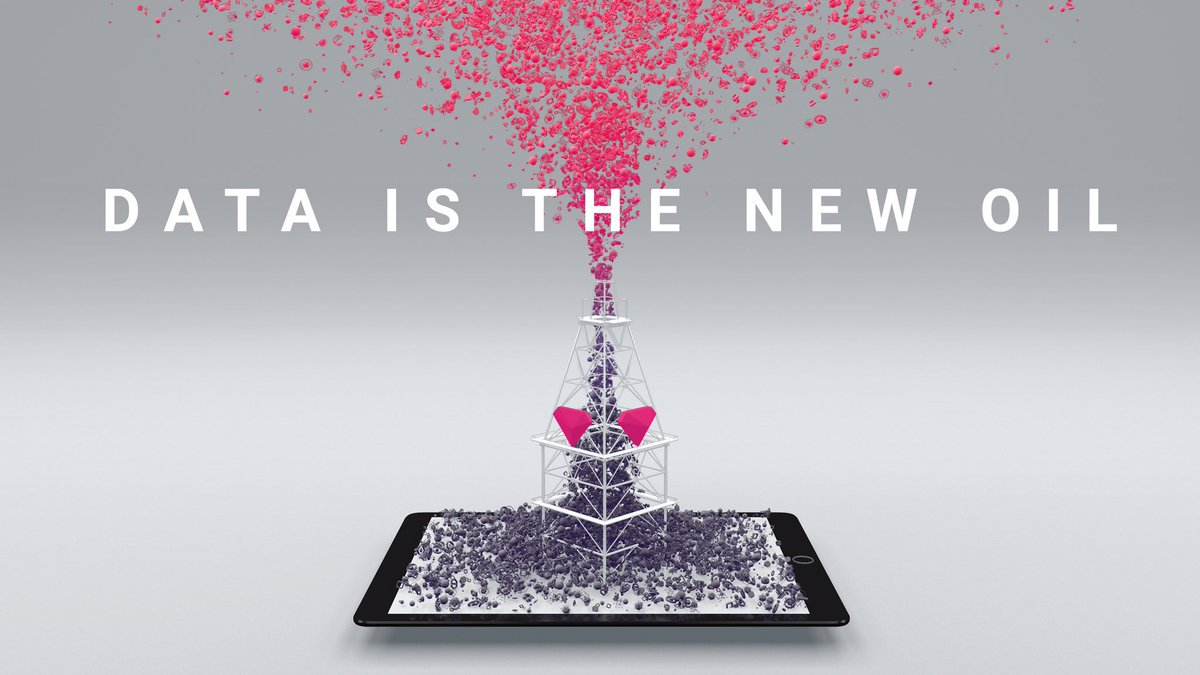
\includegraphics[scale=0.27]{Figuras/slide00_04.jpg}
\end{figure}
\scriptsize
Fonte da imagem: \href{https://bit.ly/38buOaK}{\textcolor{blue}{https://bit.ly/38buOaK}}

\end{ftst}

%===================================================================

\begin{ftst}{Importância econômica dos dados}{Ciência de dados}
\small
\begin{itemize}
    \item A informação sempre teve valor nas atividades econômicas. 
    \item No entanto, o FMI destaca duas tendências tecnológicas relativamente recentes que são essenciais para explicar o aumento estrondoso da importância dos dados - o \textbf{progresso tecnológico} e o desenvolvimento de \textbf{técnicas analíticas sofisticadas}.
    \item O progresso tecnológico reduziu drasticamente os custos de coleta, armazenamento e uso de dados quantificáveis - que, devido às atividades econômicas e sociais cada vez mais digitalizadas, estão em constante produção.
    \item O Desenvolvimento de técnicas analíticas sofisticadas possibilitou graus avançados de processamento de dados, que acrescentam valor aos dados.
\end{itemize}

\end{ftst}

%===================================================================

\begin{ftst}{Importância econômica dos dados}{Ciência de dados}
\begin{figure}
    \centering
    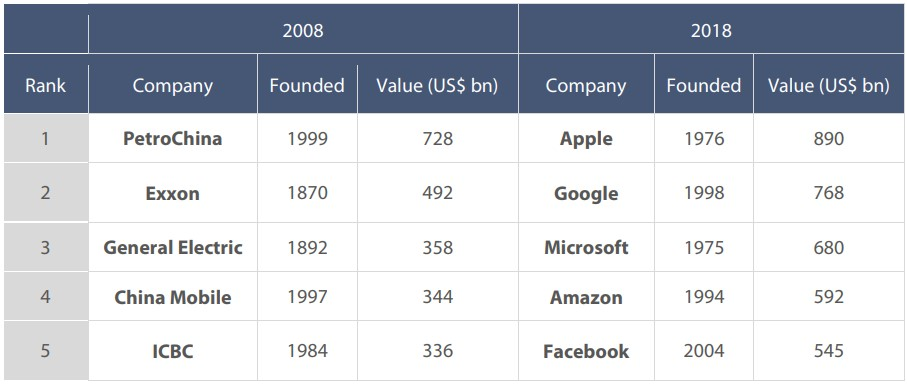
\includegraphics[scale=0.5]{Figuras/slide00_05.jpg}
\end{figure}
\vone
\vone
\vone
\scriptsize
Fonte da tabela: \href{https://bit.ly/3DcFi7M}{\textcolor{blue}{https://bit.ly/3DcFi7M}}

\end{ftst}

%===================================================================

\begin{ftst}{Um breve histórico dos bancos de dados}{Ciência de dados}
\begin{figure}
    \centering
    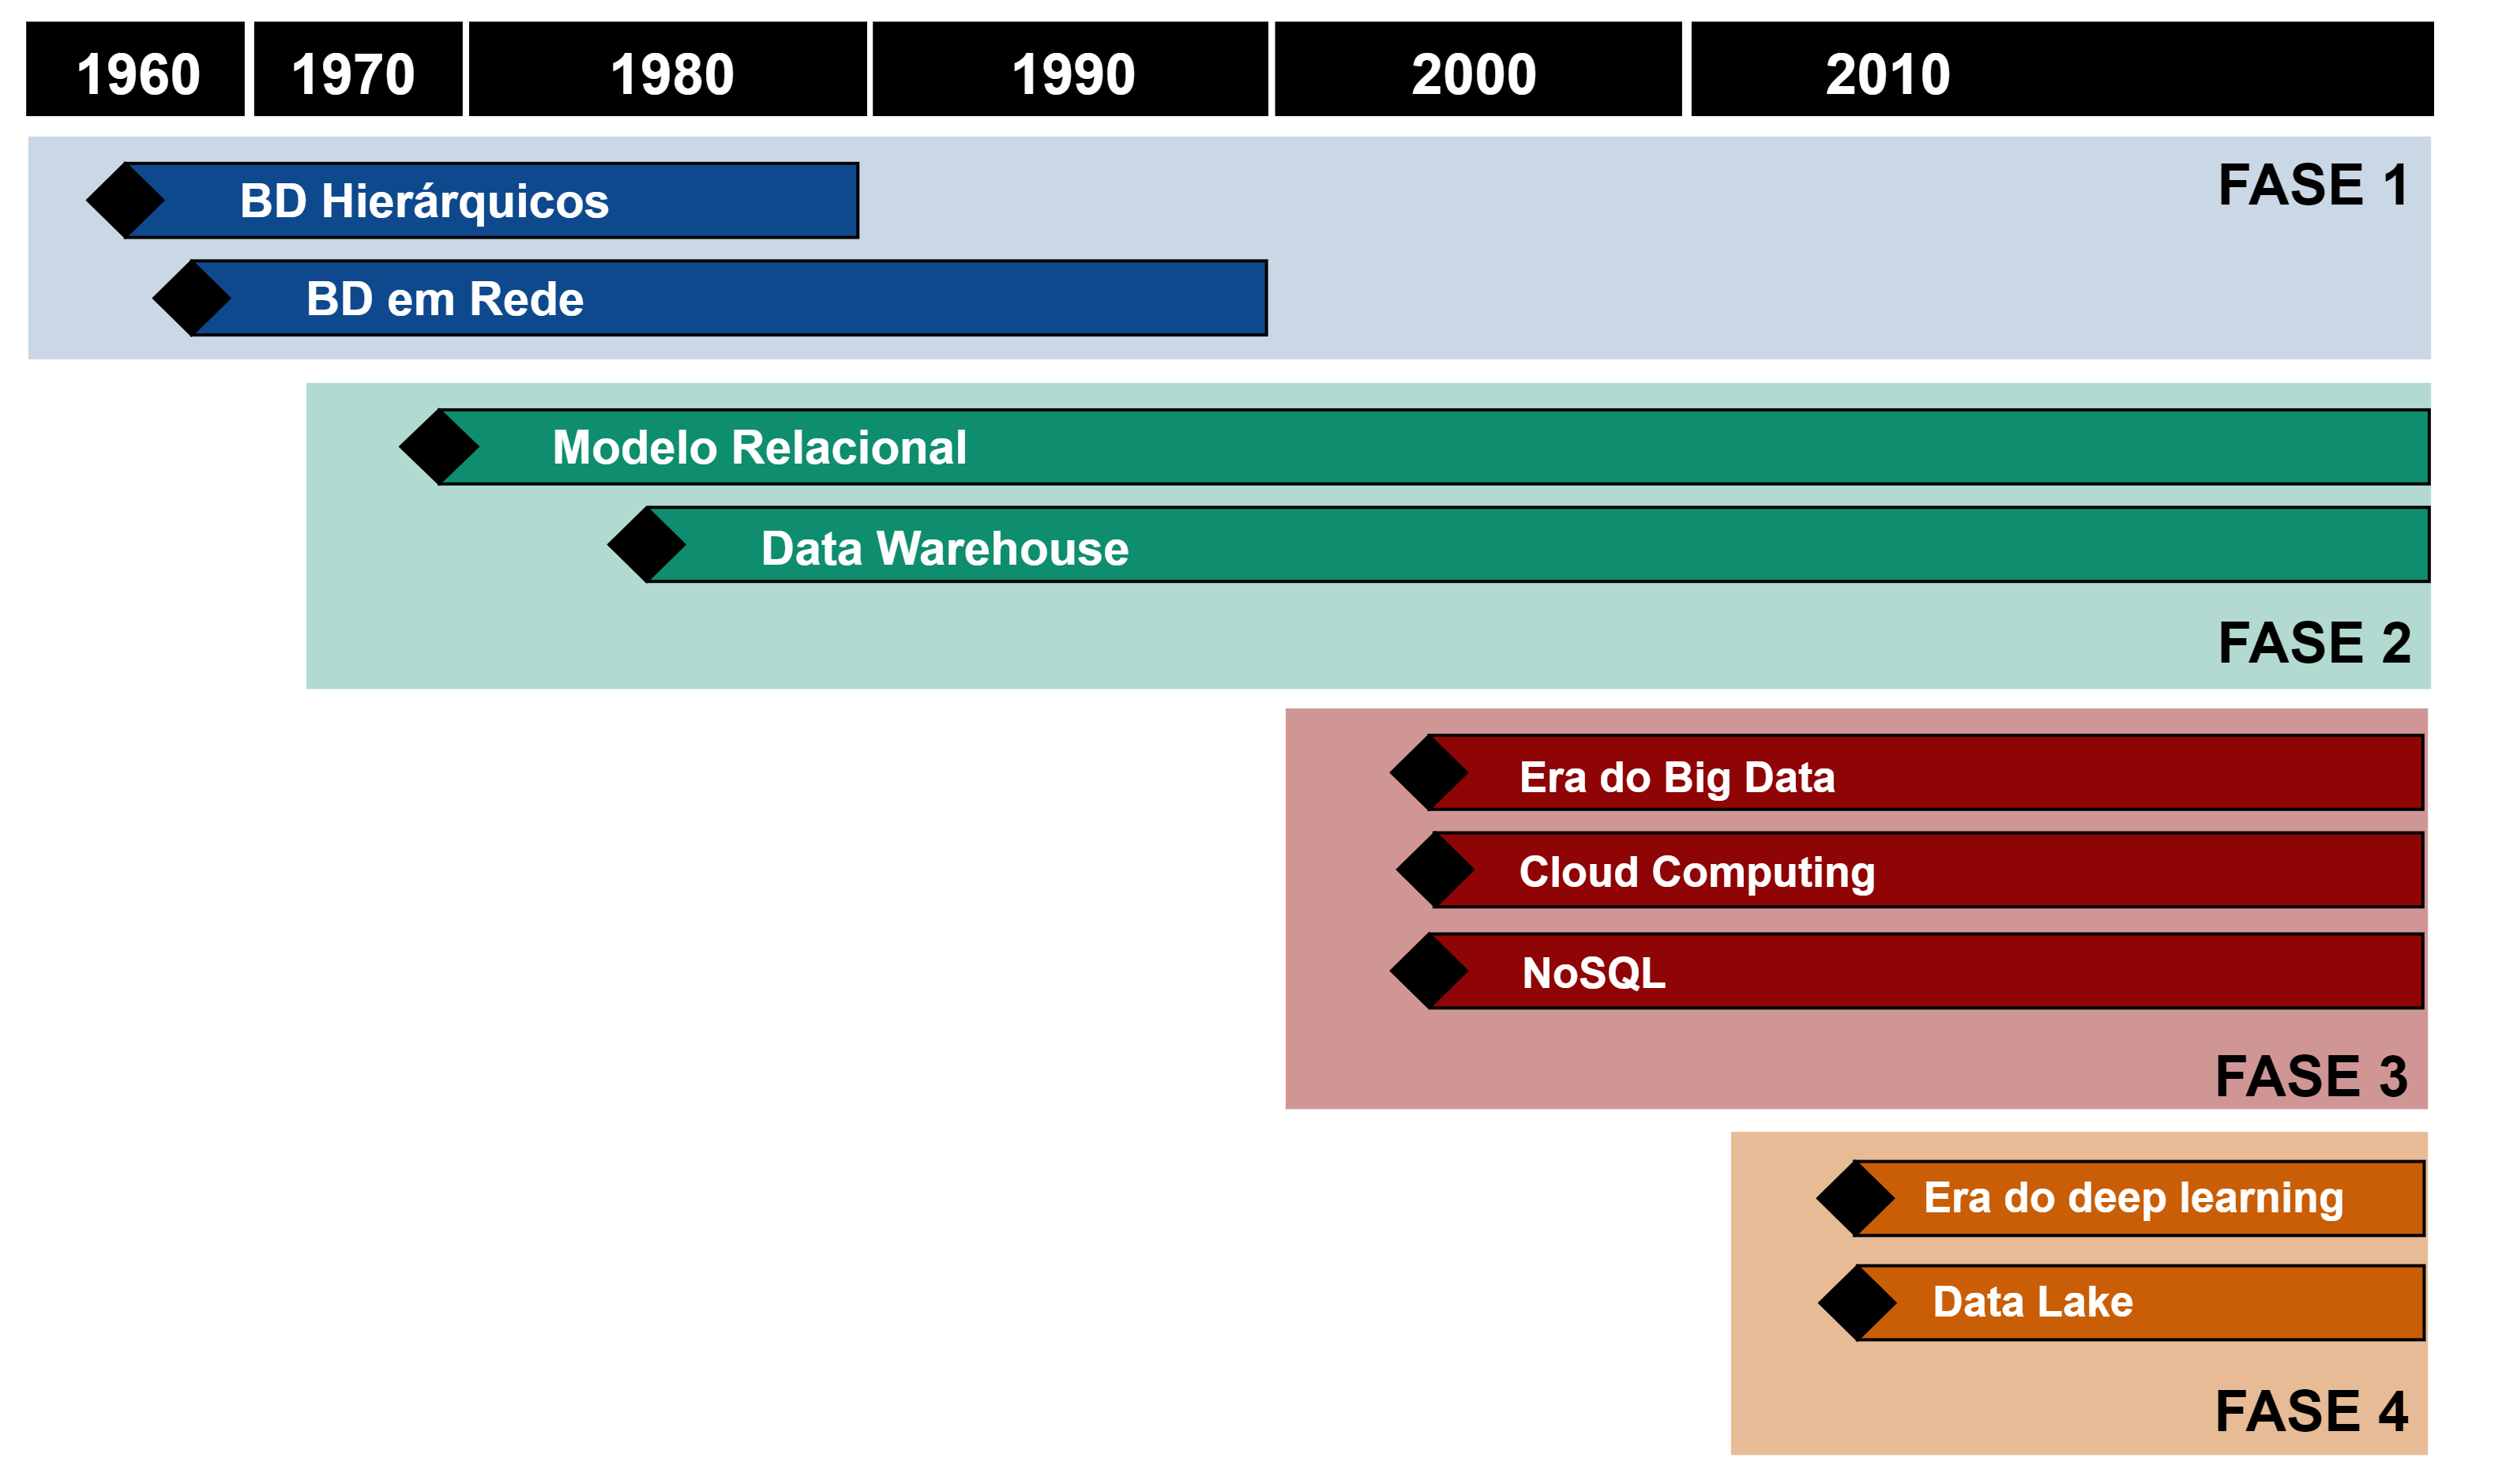
\includegraphics[scale=0.1]{Figuras/slide00_09.png}
\end{figure}
\end{ftst}
























%===================================================================

\begin{ftst}{Referências}{Ciência de dados}
\vone
\small
SZCZEPANSKI, Marcin. Is data the new oil? European Parliamentary Research Service. Janeiro, 2020. Disponível em: \href{https://www.europarl.europa.eu/RegData/etudes/BRIE/2020/646117/EPRS_BRI(2020)646117_EN.pdf.}{\textcolor{blue}{clique aqui.}}

\vone

OLIVEIRA, M; AFONSO, D. Industry Focused in Data Collection: How Industry 4.0 is Handled by Big Data. In Proceedings of the 2019 2nd International Conference on Data Science and Information Technology (DSIT 2019). Association for Computing Machinery, New York, NY, USA, 12–18. DOI:https://doi.org/10.1145/3352411.3352414. Disponível em: \href{https://dl.acm.org/doi/10.1145/3352411.3352414}{\textcolor{blue}{clique aqui.}}

\end{ftst}
\end{document}